\documentclass[aspectratio=169,10pt]{beamer}
\usetheme{metropolis}

\usepackage{graphicx}
\usepackage{booktabs}
\usepackage{tabularx}
\usepackage{array}
\usepackage{xcolor}

\title{Archived External-Detector Review}
\subtitle{Legacy H+V+V reference for afterSRC and the SAMURAI-front location}
\author{Baiting Tian}
\date{27 March 2026}

\setbeamertemplate{navigation symbols}{}

\begin{document}

\begin{frame}
  \Large \textbf{Archived External-Detector Review}

  \vspace{0.3em}
  \normalsize
  Legacy H+V+V reference snapshot from 27 March 2026

  \vspace{0.4em}
  \begin{columns}[T,onlytextwidth]
    \column{0.50\textwidth}
    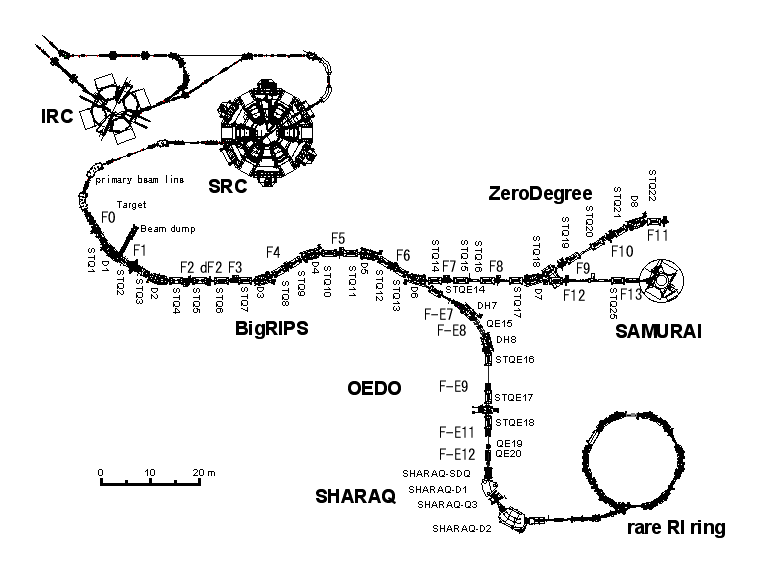
\includegraphics[width=\linewidth,height=0.24\textheight,keepaspectratio]{figures/samurai-location-map.png}

    \column{0.48\textwidth}
    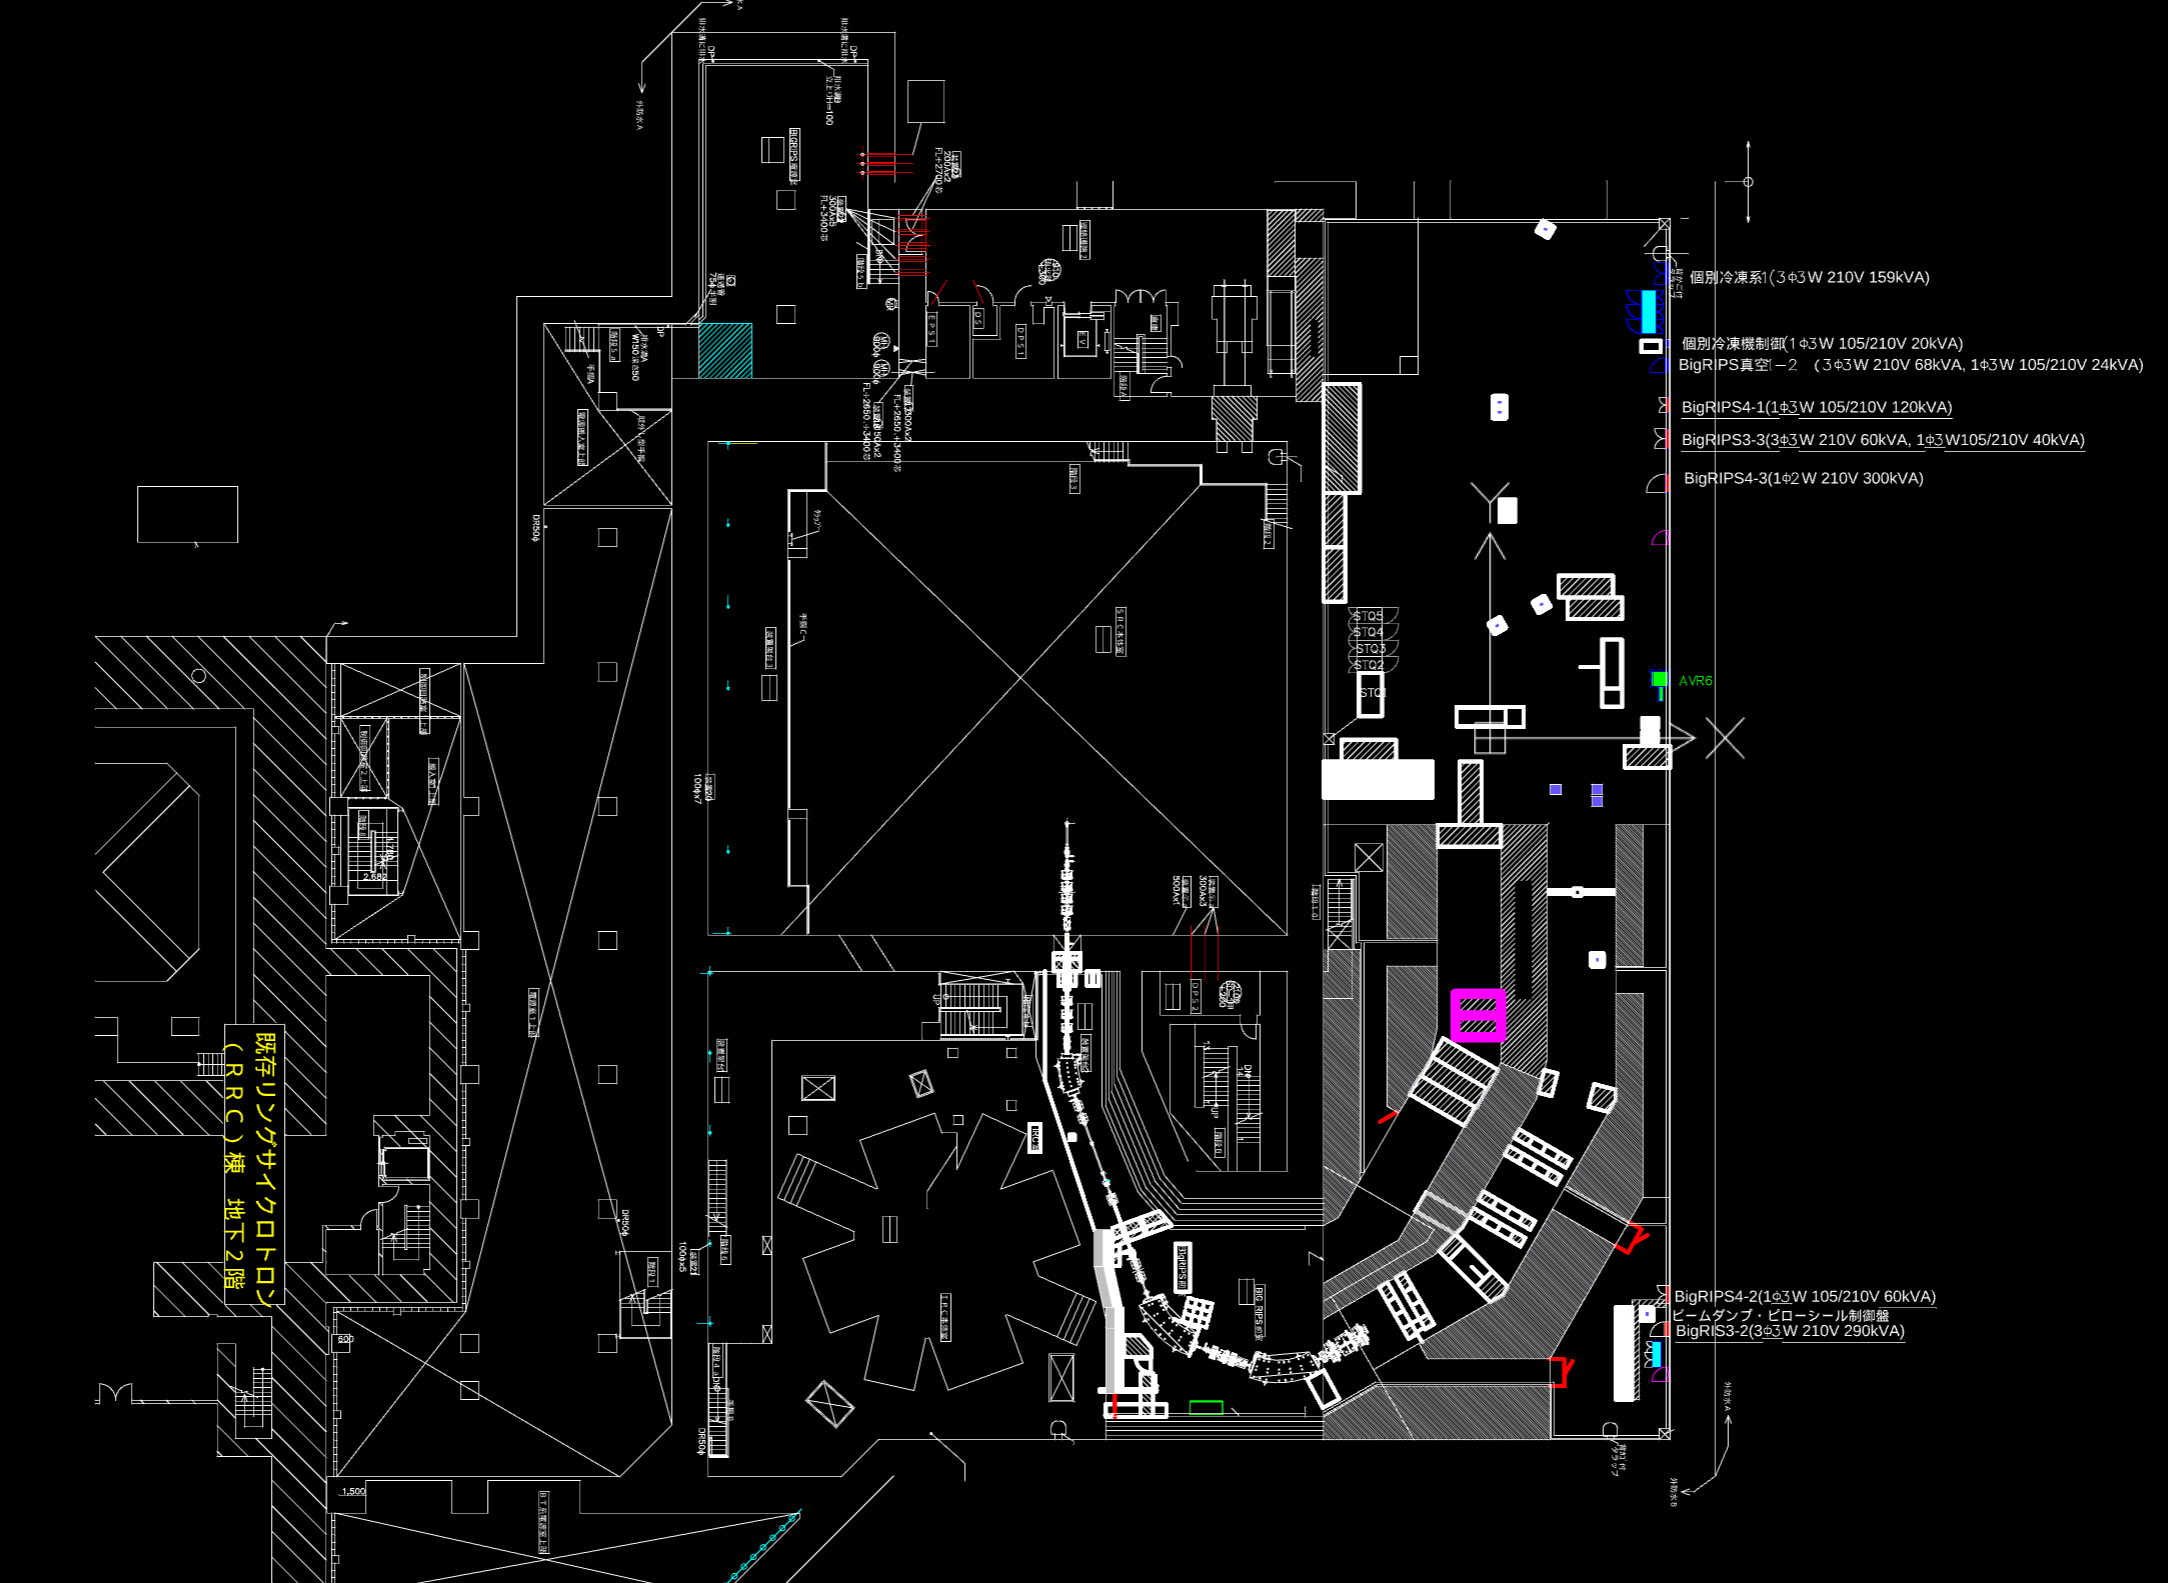
\includegraphics[width=\linewidth,height=0.24\textheight,keepaspectratio]{figures/afterSRC-context.png}
  \end{columns}

  \vspace{0.5em}
  \small
  \color{red!75!black}\bfseries
  ARCHIVED: not the current CompactInVacuum baseline and not for fabrication.

  \vspace{0.35em}
  \color{black}\normalfont
  Current requirements and CAD are controlled by
  \texttt{docs/specs/compact\_one\_requirement\_baseline.md} and
  \texttt{compactInVacuum/}.
\end{frame}

\begin{frame}{Legacy External Polarimeter at afterSRC}
  \begin{columns}[T,onlytextwidth]
    \column{0.58\textwidth}
    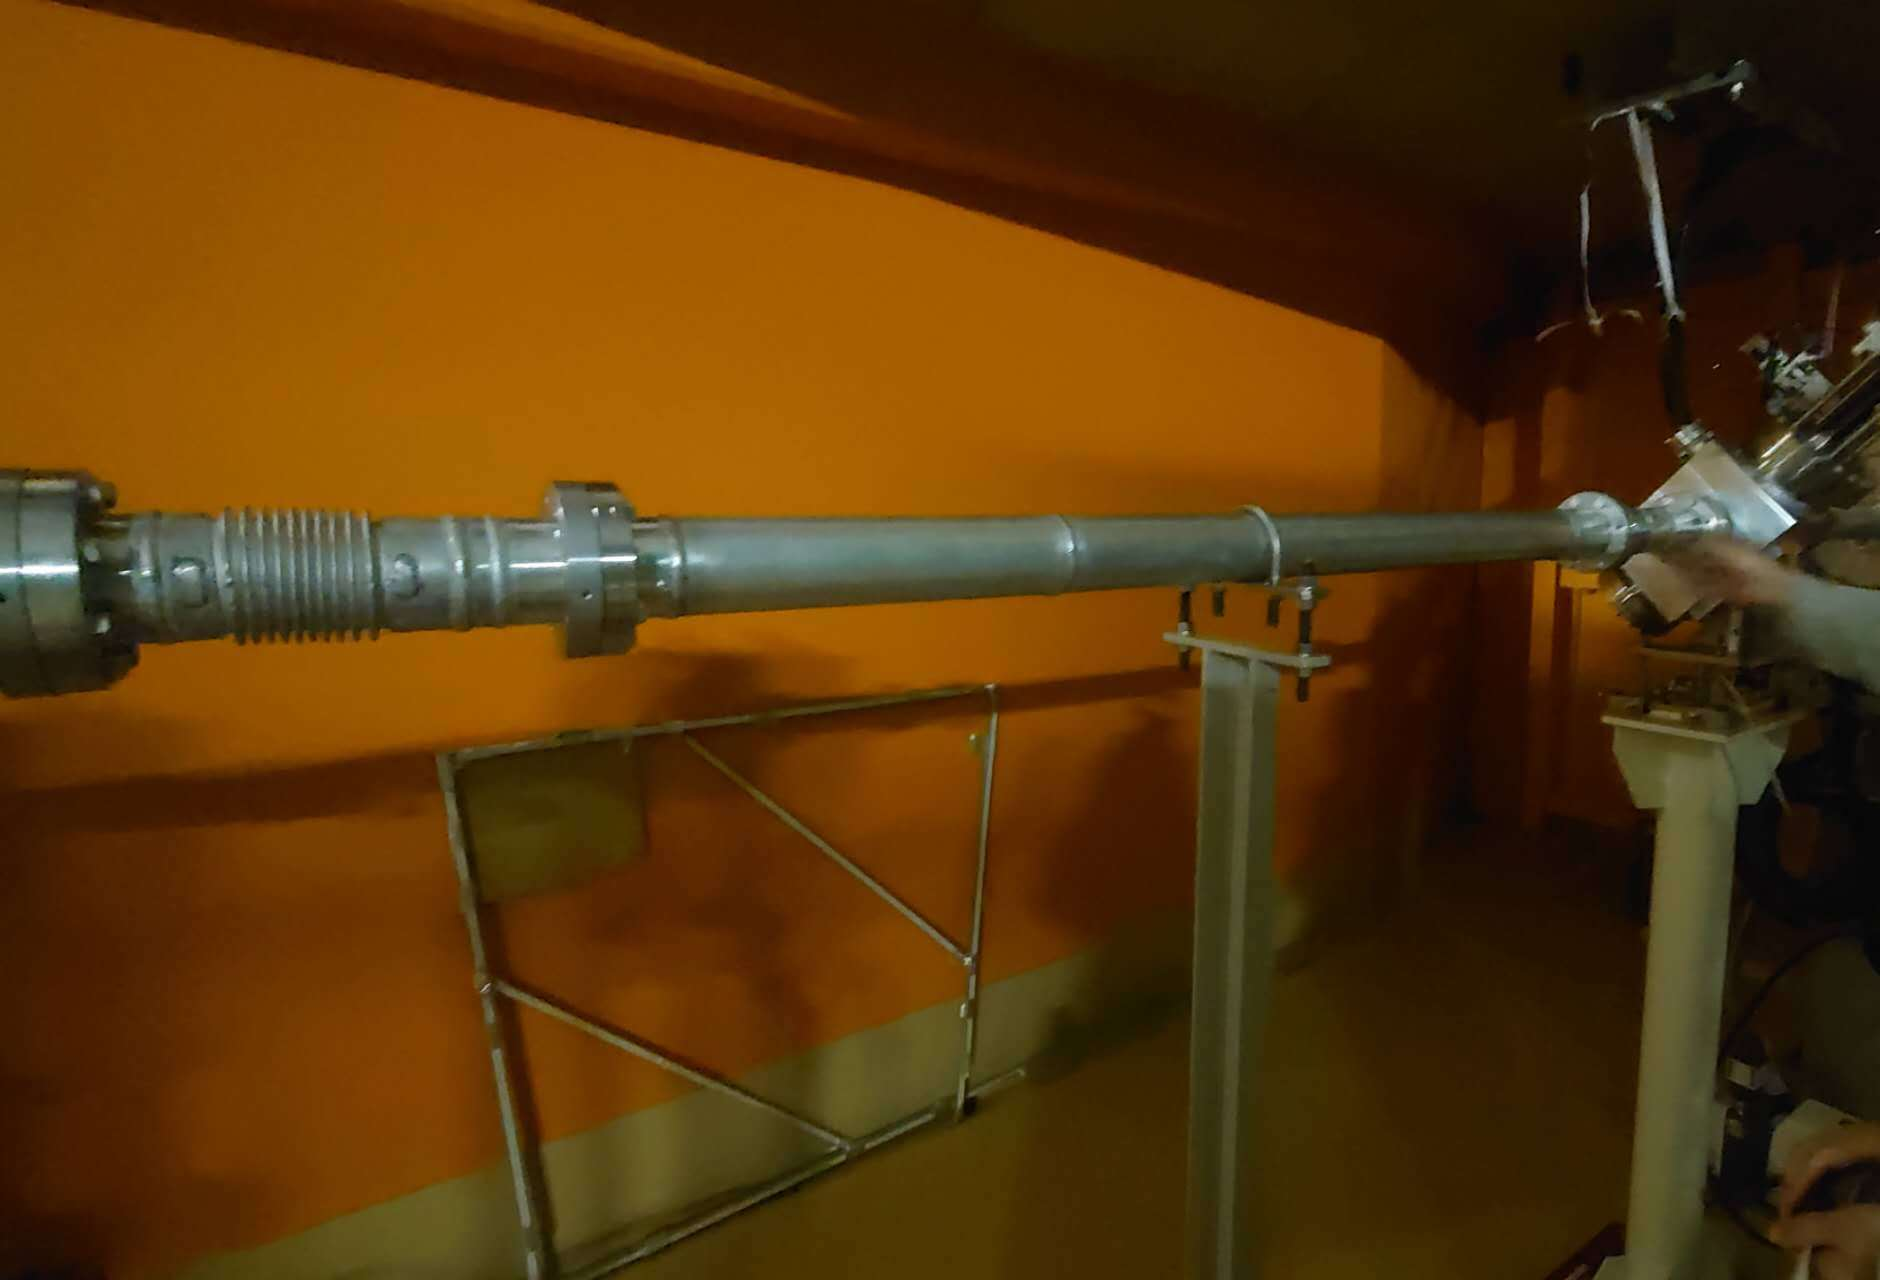
\includegraphics[width=\linewidth,height=0.64\textheight,keepaspectratio]{figures/afterSRC-layout-photo-cropped.jpg}

    \column{0.40\textwidth}
    \scriptsize
    \textbf{Role}
    \begin{itemize}
      \item Downstream polarimeter position after the SRC section.
      \item The polarimeter is organized around a dedicated target chamber.
      \item This archived concept used the external H+V+V detector arrangement.
    \end{itemize}

    \textbf{Historical interface assumptions}
    \begin{itemize}
      \item Front beam port: \texttt{ICF114}
      \item Rear beam port: \texttt{ICF114}
      \item Top rotary feedthrough mount: \texttt{ICF70}
      \item No extra side vacuum ports in this variant
    \end{itemize}
  \end{columns}
\end{frame}

\begin{frame}{Legacy External Polarimeter at the SAMURAI Side}
  \begin{columns}[T,onlytextwidth]
    \column{0.54\textwidth}
    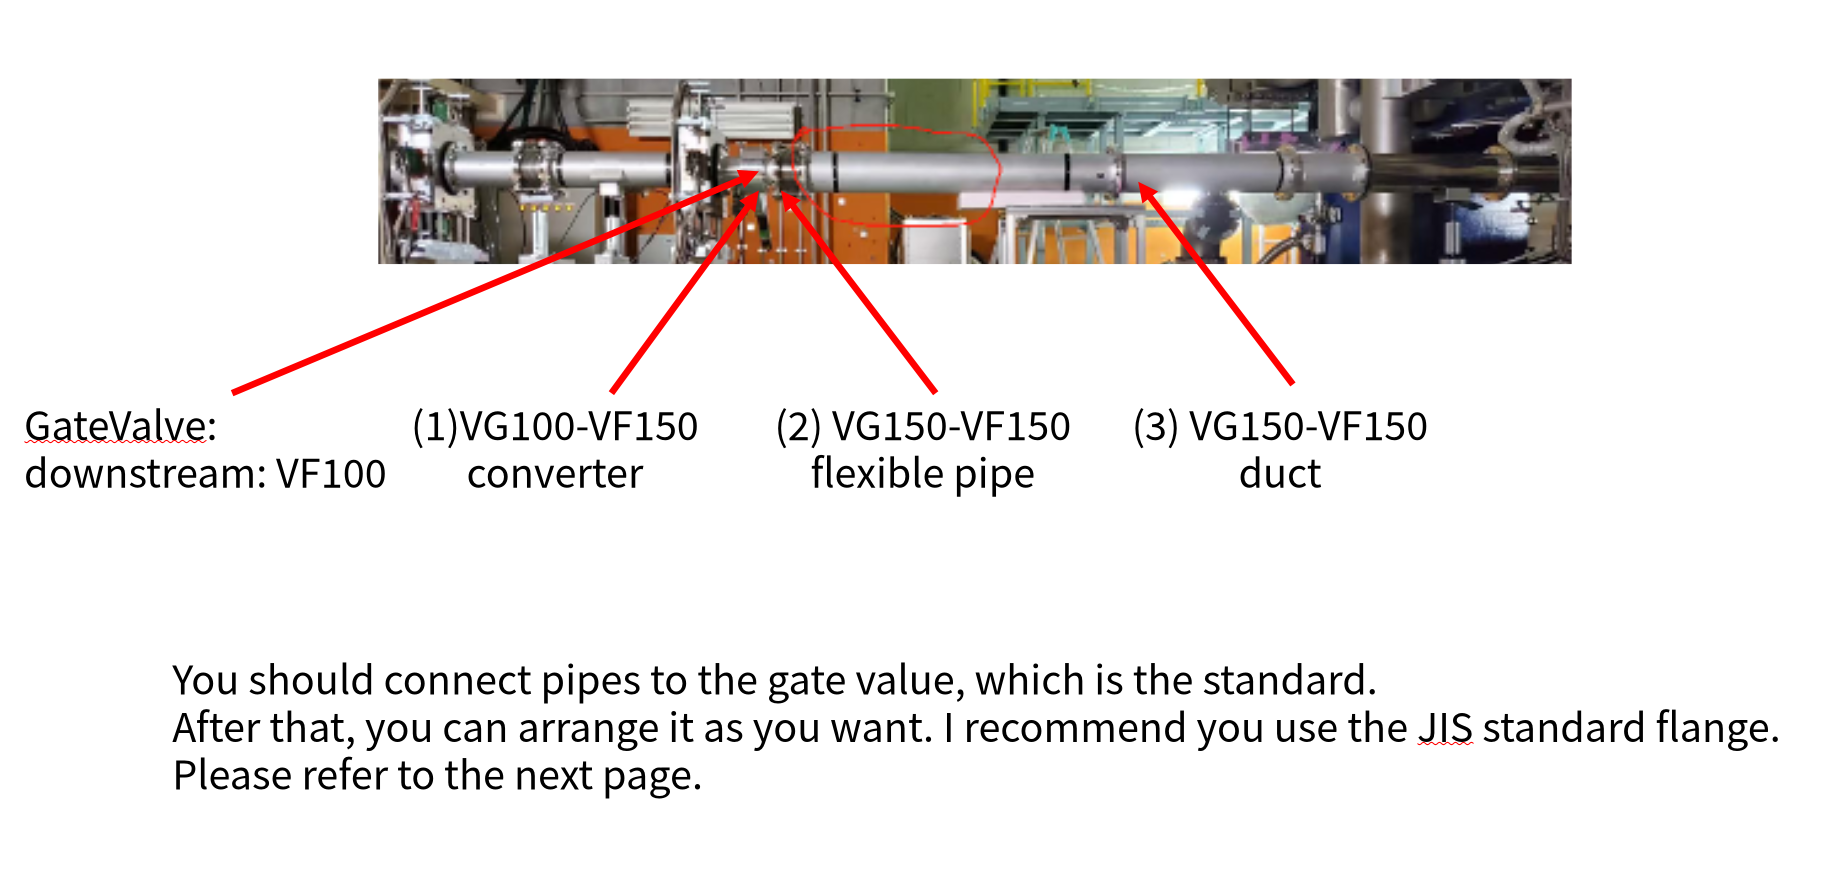
\includegraphics[width=\linewidth,height=0.27\textheight,keepaspectratio]{figures/samurai-pipe-chain.png}

    \vspace{0.3em}
    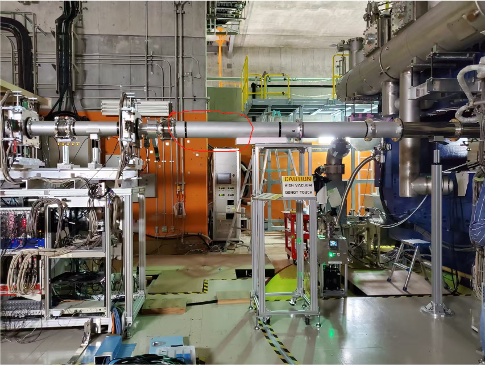
\includegraphics[width=\linewidth,height=0.19\textheight,keepaspectratio]{figures/samurai-installation-photo.png}

    \column{0.43\textwidth}
    \tiny
    \textbf{Role}
    \begin{itemize}
      \item A SAMURAI-side polarimeter option is integration-driven rather than chamber-driven.
      \item The immediate boundary is defined by the beam pipe, the gate valve, and the local installation envelope.
    \end{itemize}

    \textbf{Historical interface understanding}
    \begin{itemize}
      \item Local standard family: \textbf{JIS} vacuum flanges and pipe-chain hardware
      \item Fixed gate-valve boundary at the local downstream side: \texttt{JIS VF100}
      \item Transition pipe (1): \texttt{JIS VG100--VF150} converter
      \item Transition pipe (2): \texttt{JIS VG150--VF150} flexible pipe
      \item Transition pipe (3): \texttt{JIS VG150--VF150} rigid duct
      \item Local space and maintenance envelope remain the dominant constraints for the upstream / in-front-of-SAMURAI polarimeter option
    \end{itemize}
  \end{columns}
\end{frame}

\begin{frame}{Archived afterSRC External Design}
  \begin{columns}[T,onlytextwidth]
    \column{0.58\textwidth}
    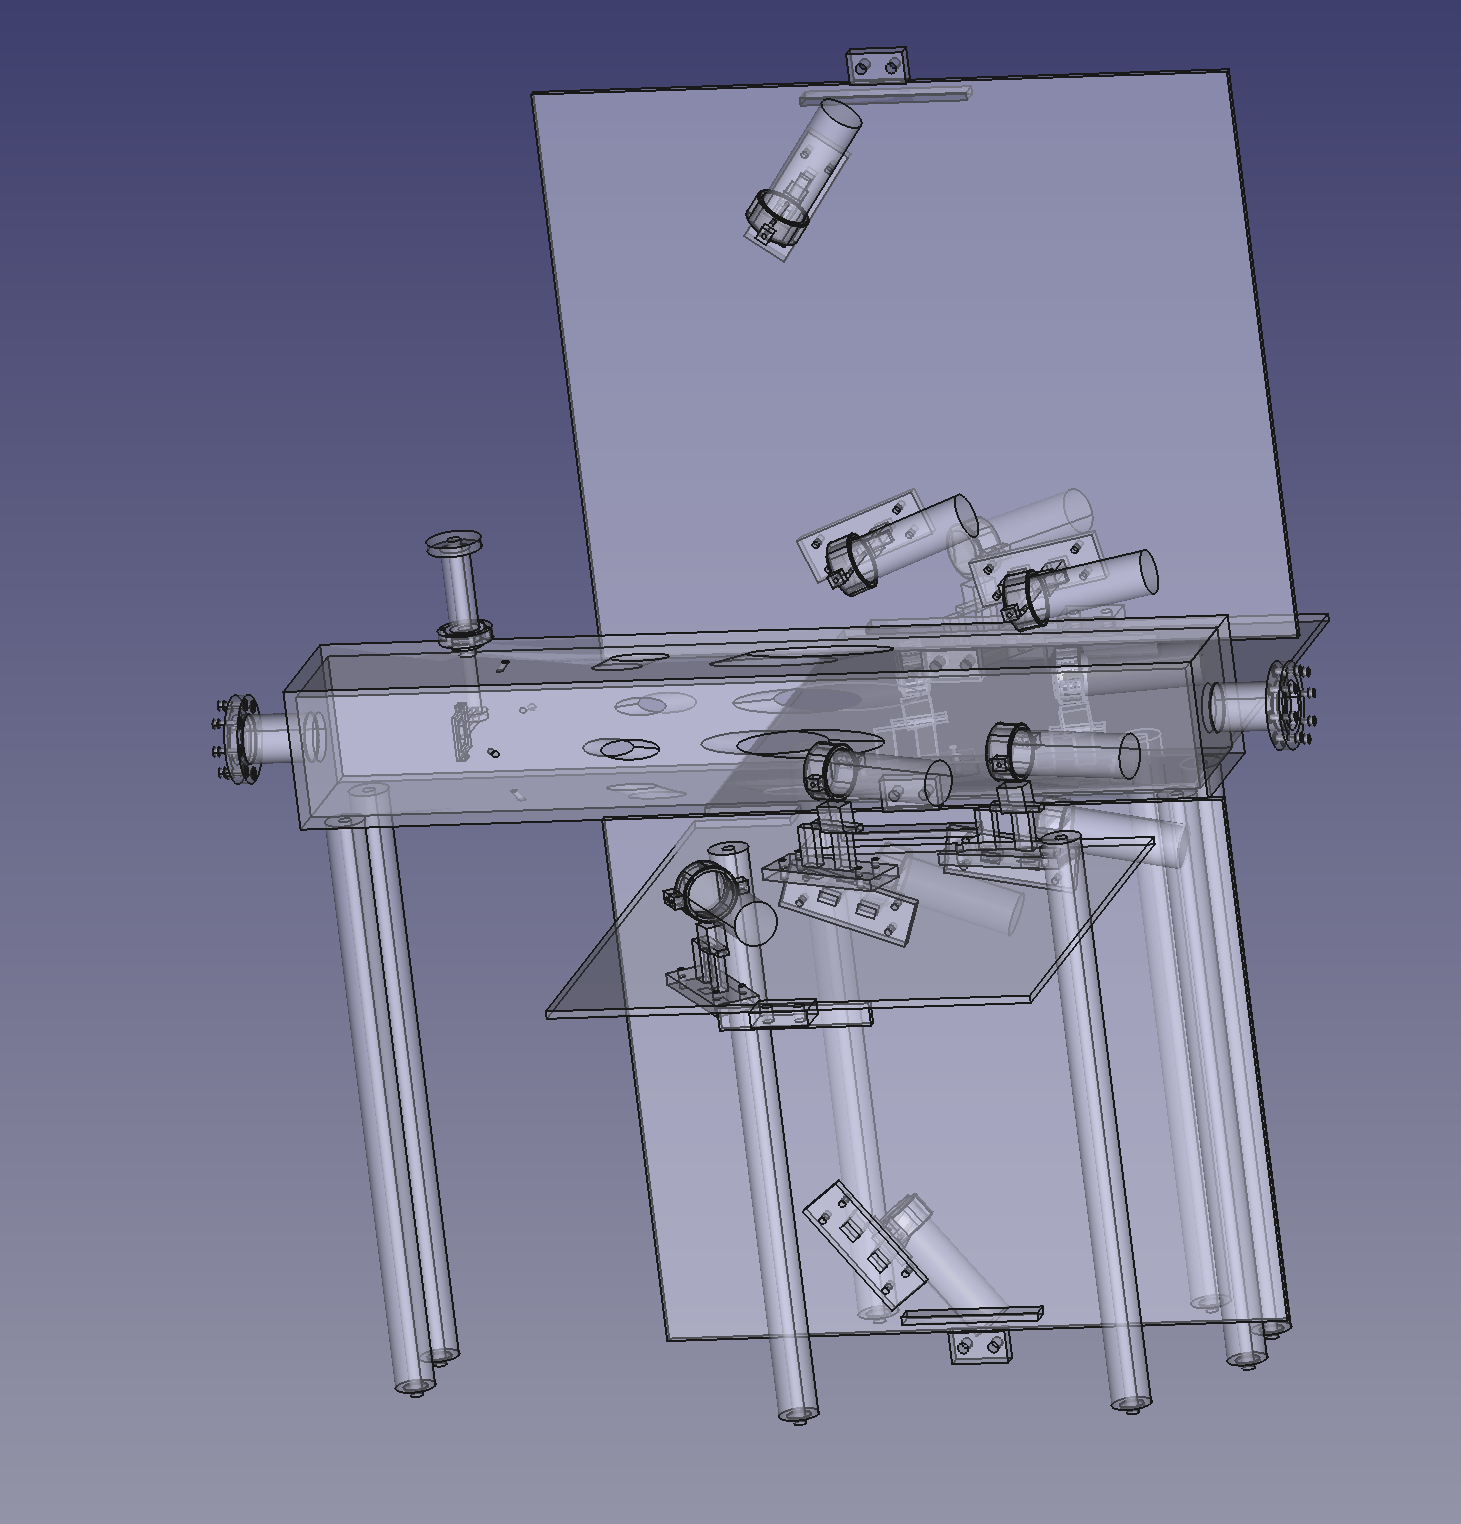
\includegraphics[width=\linewidth,height=0.60\textheight,keepaspectratio]{figures/2026-03-27-10-16-38.png}

    \column{0.39\textwidth}
    \tiny
    \textbf{Historical interfaces visible in this view}
    \begin{itemize}
      \item Front beamline interface: \texttt{ICF114} CF flange for the upstream beam connection
      \item Rear beamline interface: \texttt{ICF114} CF flange for the downstream beam connection
      \item Top target-drive interface: \texttt{ICF70} CF flange for the rotary feedthrough
      \item The chamber body is welded to short round beam pipes so the upstream and downstream beamline vacuum can be kept continuous after installation
    \end{itemize}

    \textbf{Legacy layout note}
    \begin{itemize}
      \item This image belongs to the preserved external-detector reference route; it does not describe the current in-vacuum baseline
    \end{itemize}

    \textbf{Fabrication-status correction}

    \vspace{0.25em}
    The LOS openings shown here were \textbf{temporary visualization cuts} in the archived model.

    \vspace{0.35em}
    No wall-thinning or cutout statement from this deck is approved for fabrication. Any retained
    external-route chamber must be re-evaluated against the legacy baseline, vacuum boundary,
    external-pressure calculation, weld design, and current validation evidence.
  \end{columns}
\end{frame}

\begin{frame}{Archived SAMURAI-front External Design}
  \begin{columns}[T,onlytextwidth]
    \column{0.58\textwidth}
    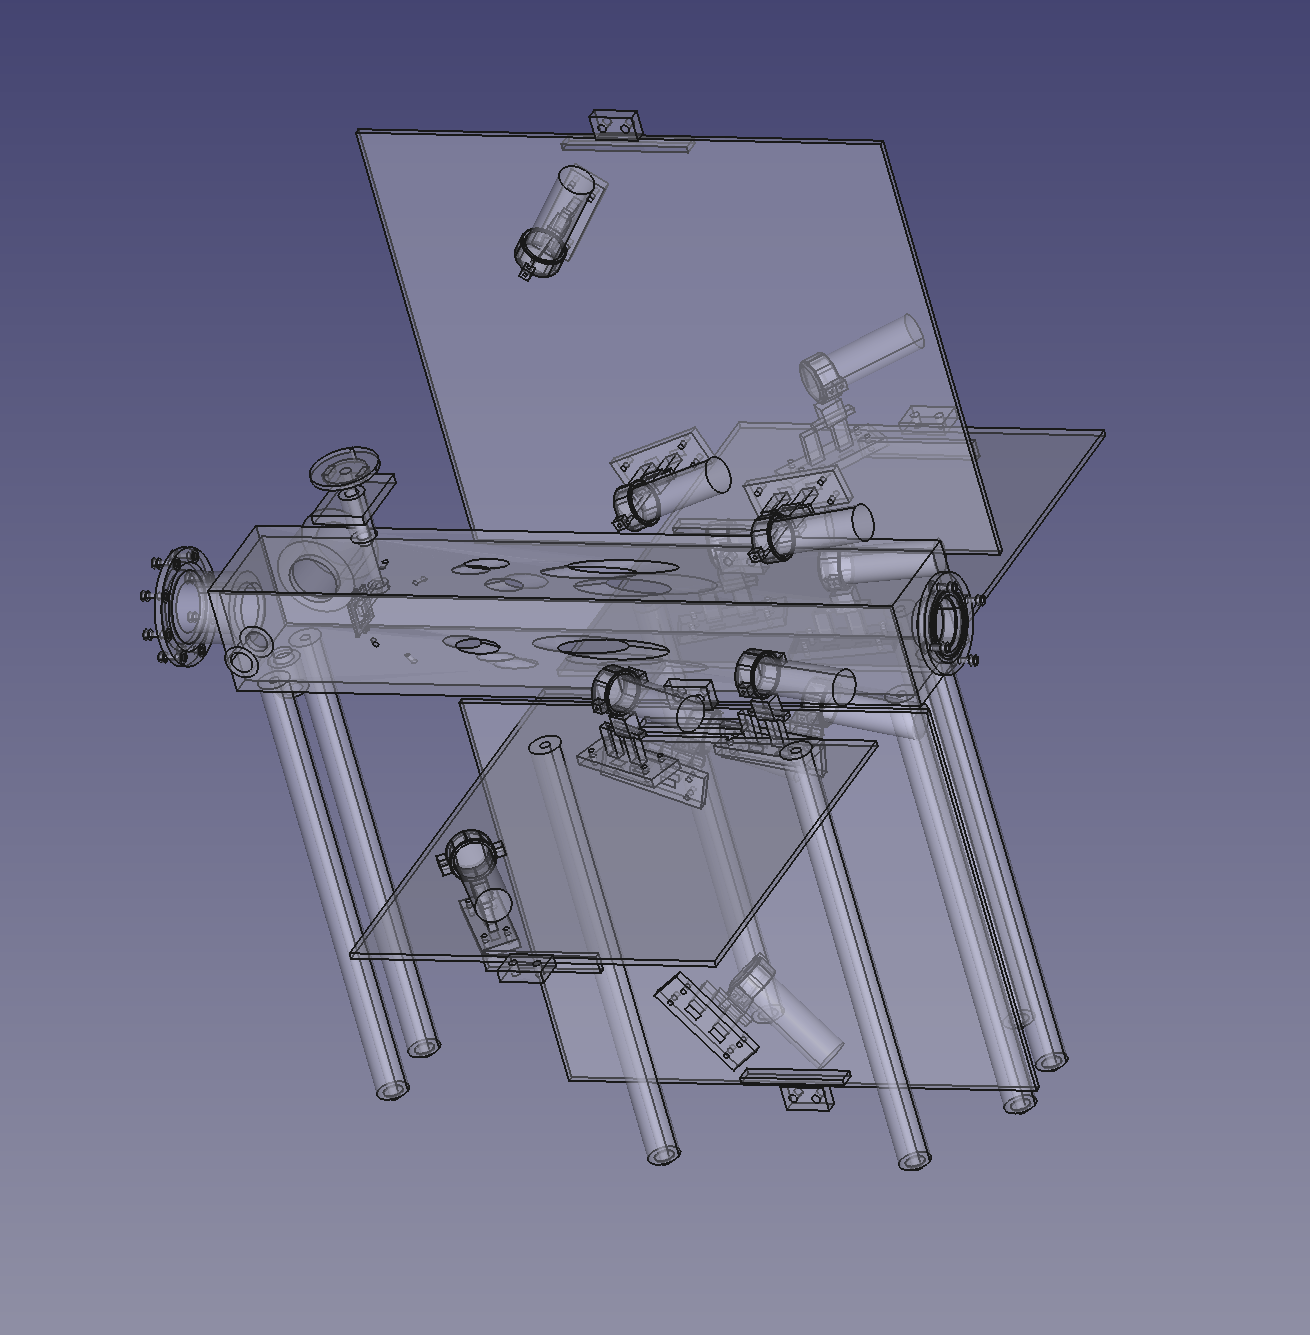
\includegraphics[width=\linewidth,height=0.64\textheight,keepaspectratio]{figures/2026-03-27-10-18-22.png}

    \column{0.39\textwidth}
    \scriptsize
    \textbf{Historical interface interpretation}
    \begin{itemize}
      \item The SAMURAI-side mechanical interface follows the existing \textbf{JIS} beam-pipe standard rather than the ICF chamber style used at afterSRC
      \item Fixed local beamline boundary at the gate valve: \texttt{JIS VF100}
      \item Required transition pieces in the present understanding are \texttt{JIS VG100--VF150}, then \texttt{JIS VG150--VF150} flexible and rigid sections
    \end{itemize}

    \textbf{Mechanical consequence}
    \begin{itemize}
      \item This option must be sized around the existing valve, pipe, and maintenance envelope close to SAMURAI
      \item Interface definition and available straight length remain the primary constraints for the final detector-side adapter geometry
    \end{itemize}
  \end{columns}
\end{frame}

\end{document}
